\documentclass{article}
\usepackage[margin=1in]{geometry}
\usepackage{amsmath,amssymb,booktabs,multirow,graphicx}
\usepackage{xcolor}
\usepackage[colorlinks=true,citecolor=blue]{hyperref}

\newcommand{\R}{\mathbb{R}}
\newcommand{\gN}{\mathcal{N}}
\newcommand{\ess}{\text{ESS}}

\begin{document}

\section{Cosmology: DES Y1 \texorpdfstring{$3\times 2$pt}{3x2pt}}\label{sec:desY1}

\emph{Scope note.} This is the PICKLES-focused note: the headline
comparison is Metropolized PICKLES against NUTS (\texttt{NumPyro}) and
\texttt{emcee}. All gradient-sampler results use the corrected
step-size dual-averaging (Nesterov gain $\sqrt m/\gamma$); see
\texttt{results/des\_y1\_fda/} for the directory-to-table map.

We benchmark on the Dark Energy Survey Year~1 (DES~Y1) $3\times 2$pt
cosmological inference, implemented through the \texttt{JAX-COSMO}
forward model. The posterior is $D=21$ dimensional, with the standard
cosmology reparametrization (logit transform on the 13 Uniform priors
and non-centered location-scale on the 8 Gaussian priors), so the prior
is $\gN(0,I_{21})$ in the sampled $z$-space. Empirically the posterior
has condition number $\kappa(\Sigma)\!\approx\!300$, with six parameter
pairs at $|\rho|>0.9$ --- all between $\sigma_8$ and the five galaxy
bias parameters $b_{1\!:\!5}$ --- and eight prior-dominated nuisance
directions (Figure~\ref{fig:desCorner}). PICKLES uses the empirical
covariance of the live walker ensemble as a preconditioner, recomputed
every iteration, in place of a separately-adapted mass matrix; its two
tuning knobs are the kinetic-damping coefficient $\gamma$ and the
trajectory-length cap $L_{\max}$.

All runs use float64 on a single NVIDIA H100 GPU. ESS denotes the
minimum effective sample size across the $21$ dimensions, from the
uncapped integrated autocorrelation time ($\hat\tau<1$ allowed for
antithetic chains); ESS\,/\,eval is the production-only count of target
evaluations (gradients for HMC/PICKLES, log-probs for \texttt{emcee}).
PICKLES rows are $3$-seed medians at $N{=}1000$ (single seed at
$N{=}5000$); NUTS uses deterministic \texttt{init\_to\_median}.

\begin{figure}[t]
\centering
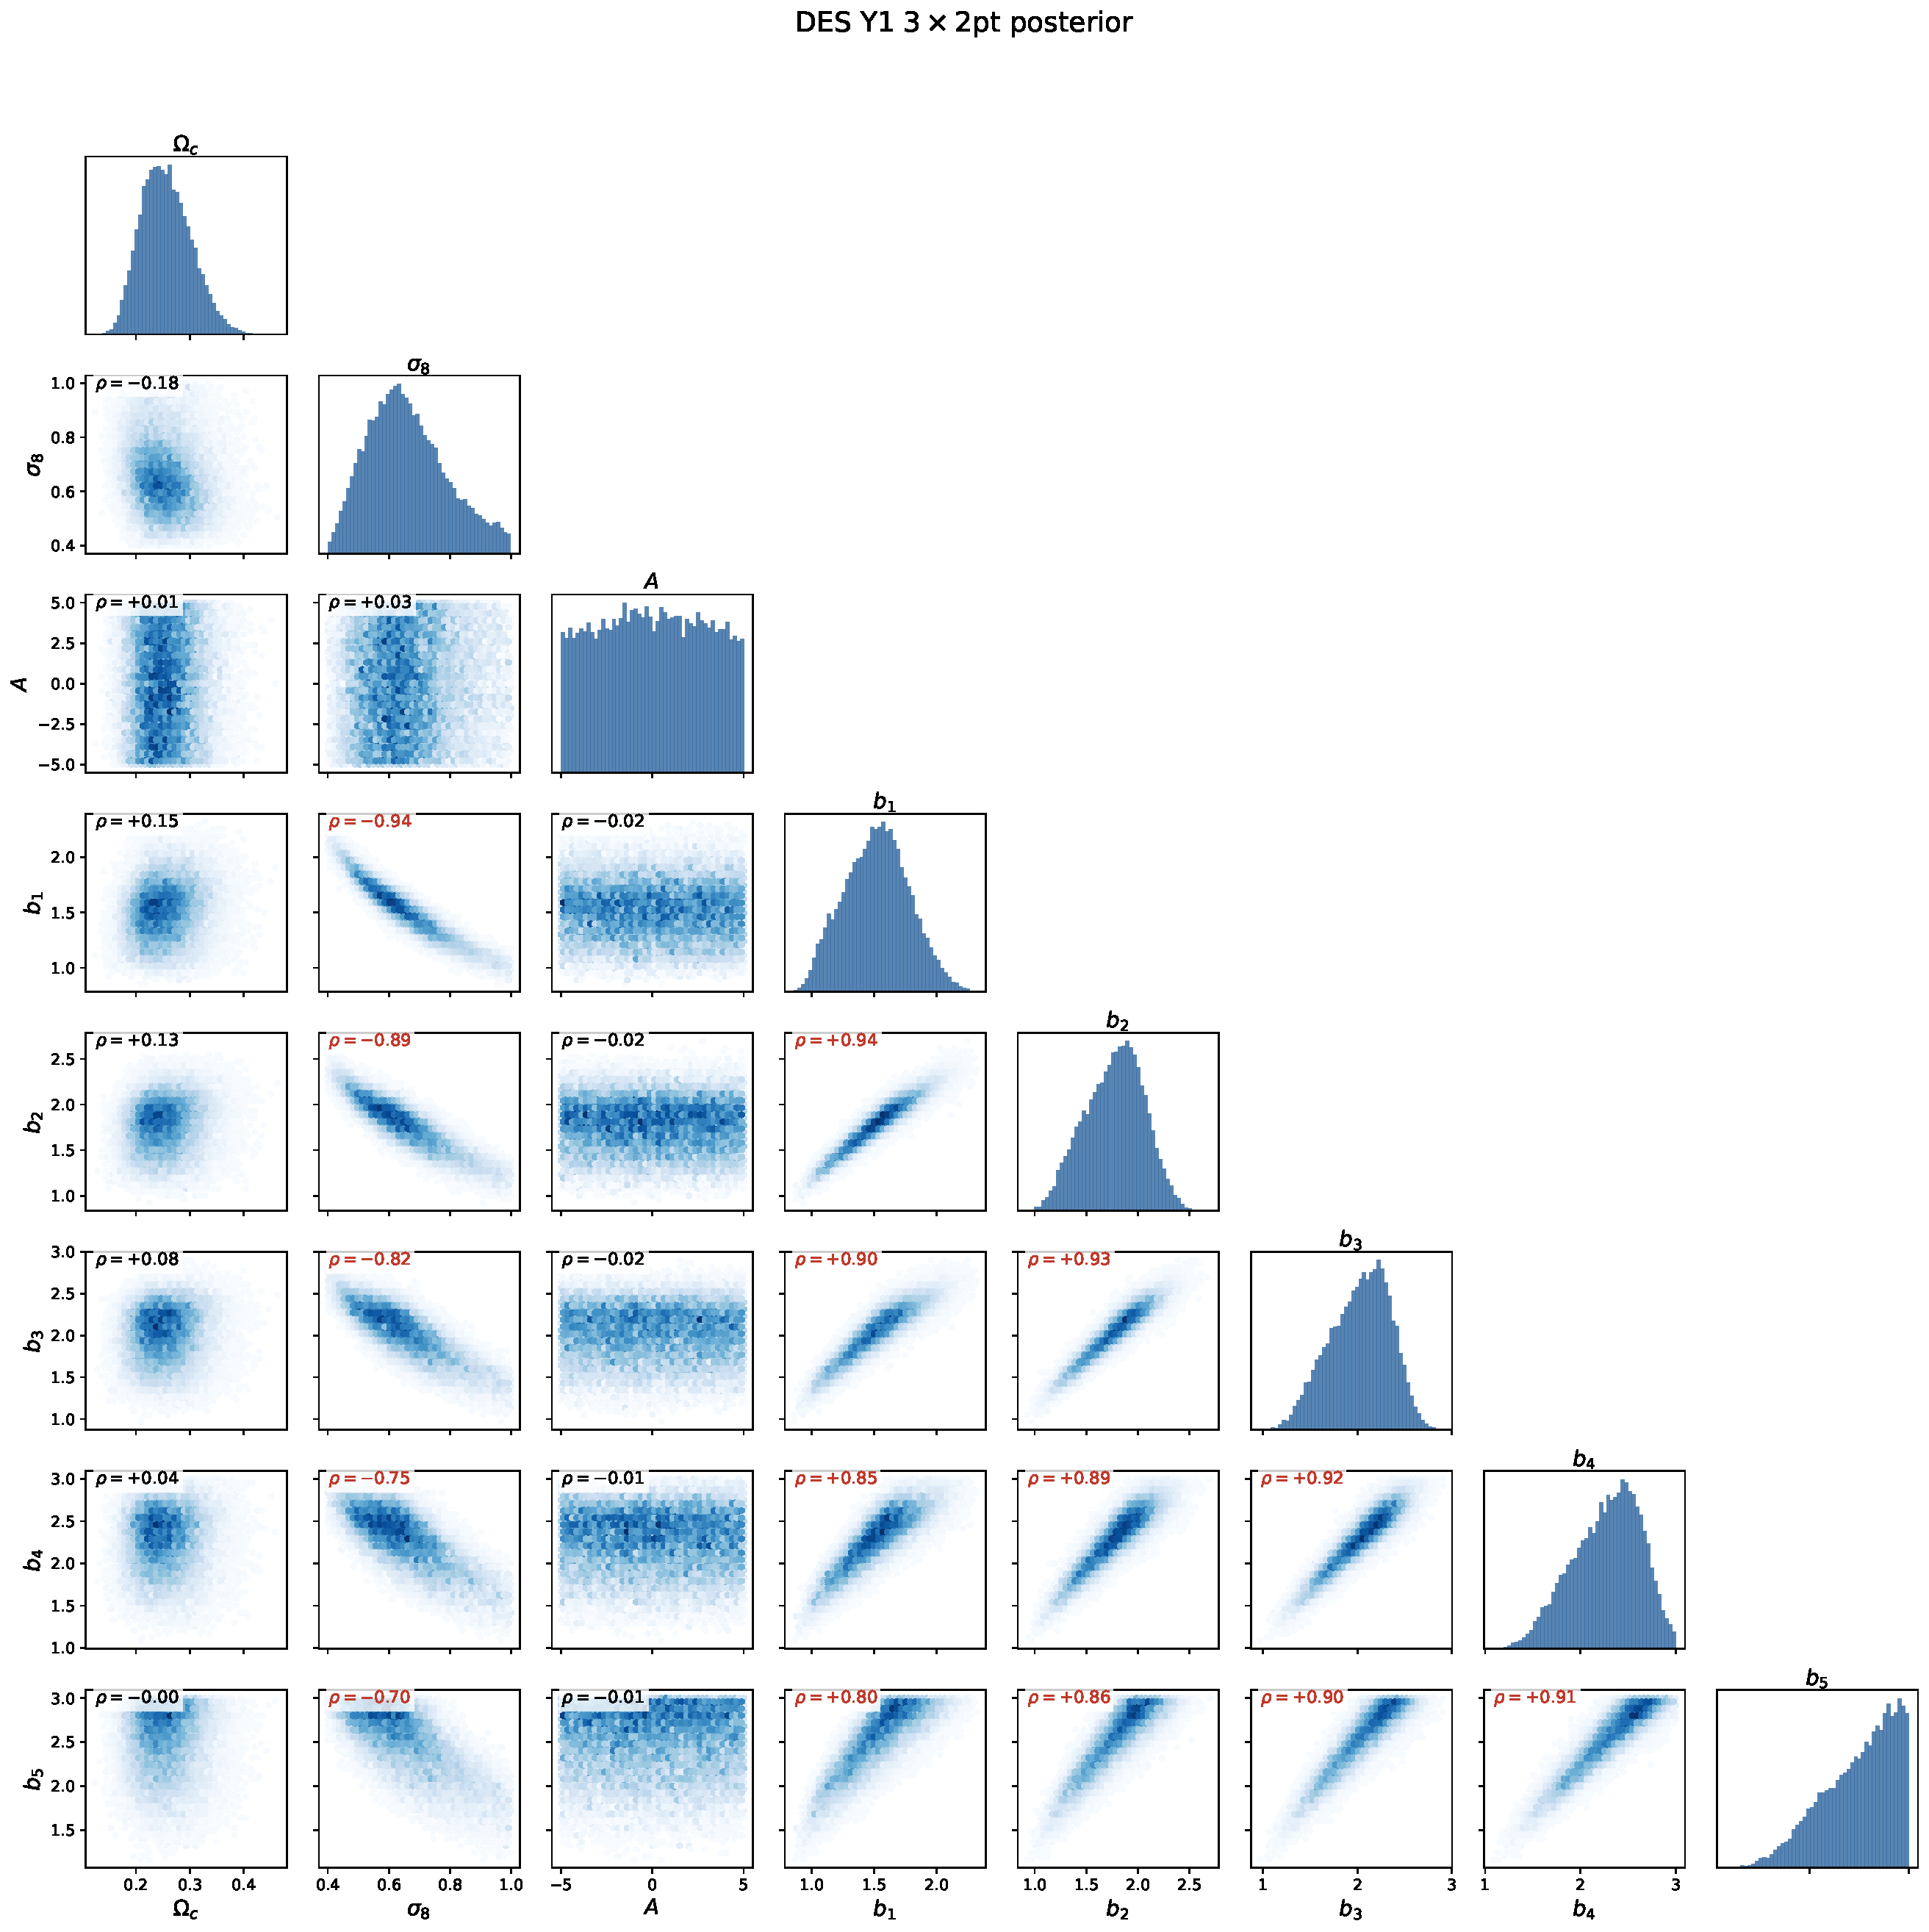
\includegraphics[width=0.95\linewidth]{figs/des_y1_corner_optB.pdf}
\caption{DES~Y1 $3\times 2$pt posterior, eight \emph{sampled}
marginals of $D=21$. The control panels (rows $\Omega_c$, $A$) show
near-isotropic ellipses with $|\rho|\le0.2$, while every panel
involving $\sigma_8$ and the five galaxy biases $b_{1:5}$ shows a narrow
ridge ($|\rho|$ from $0.70$ to $0.94$). The slow-mixing $6$-dim subspace
consists entirely of $\sigma_8+b_{1:5}$ (\S\ref{ssec:desPerDim}).}
\label{fig:desCorner}
\end{figure}

\begin{figure}[t]
\centering
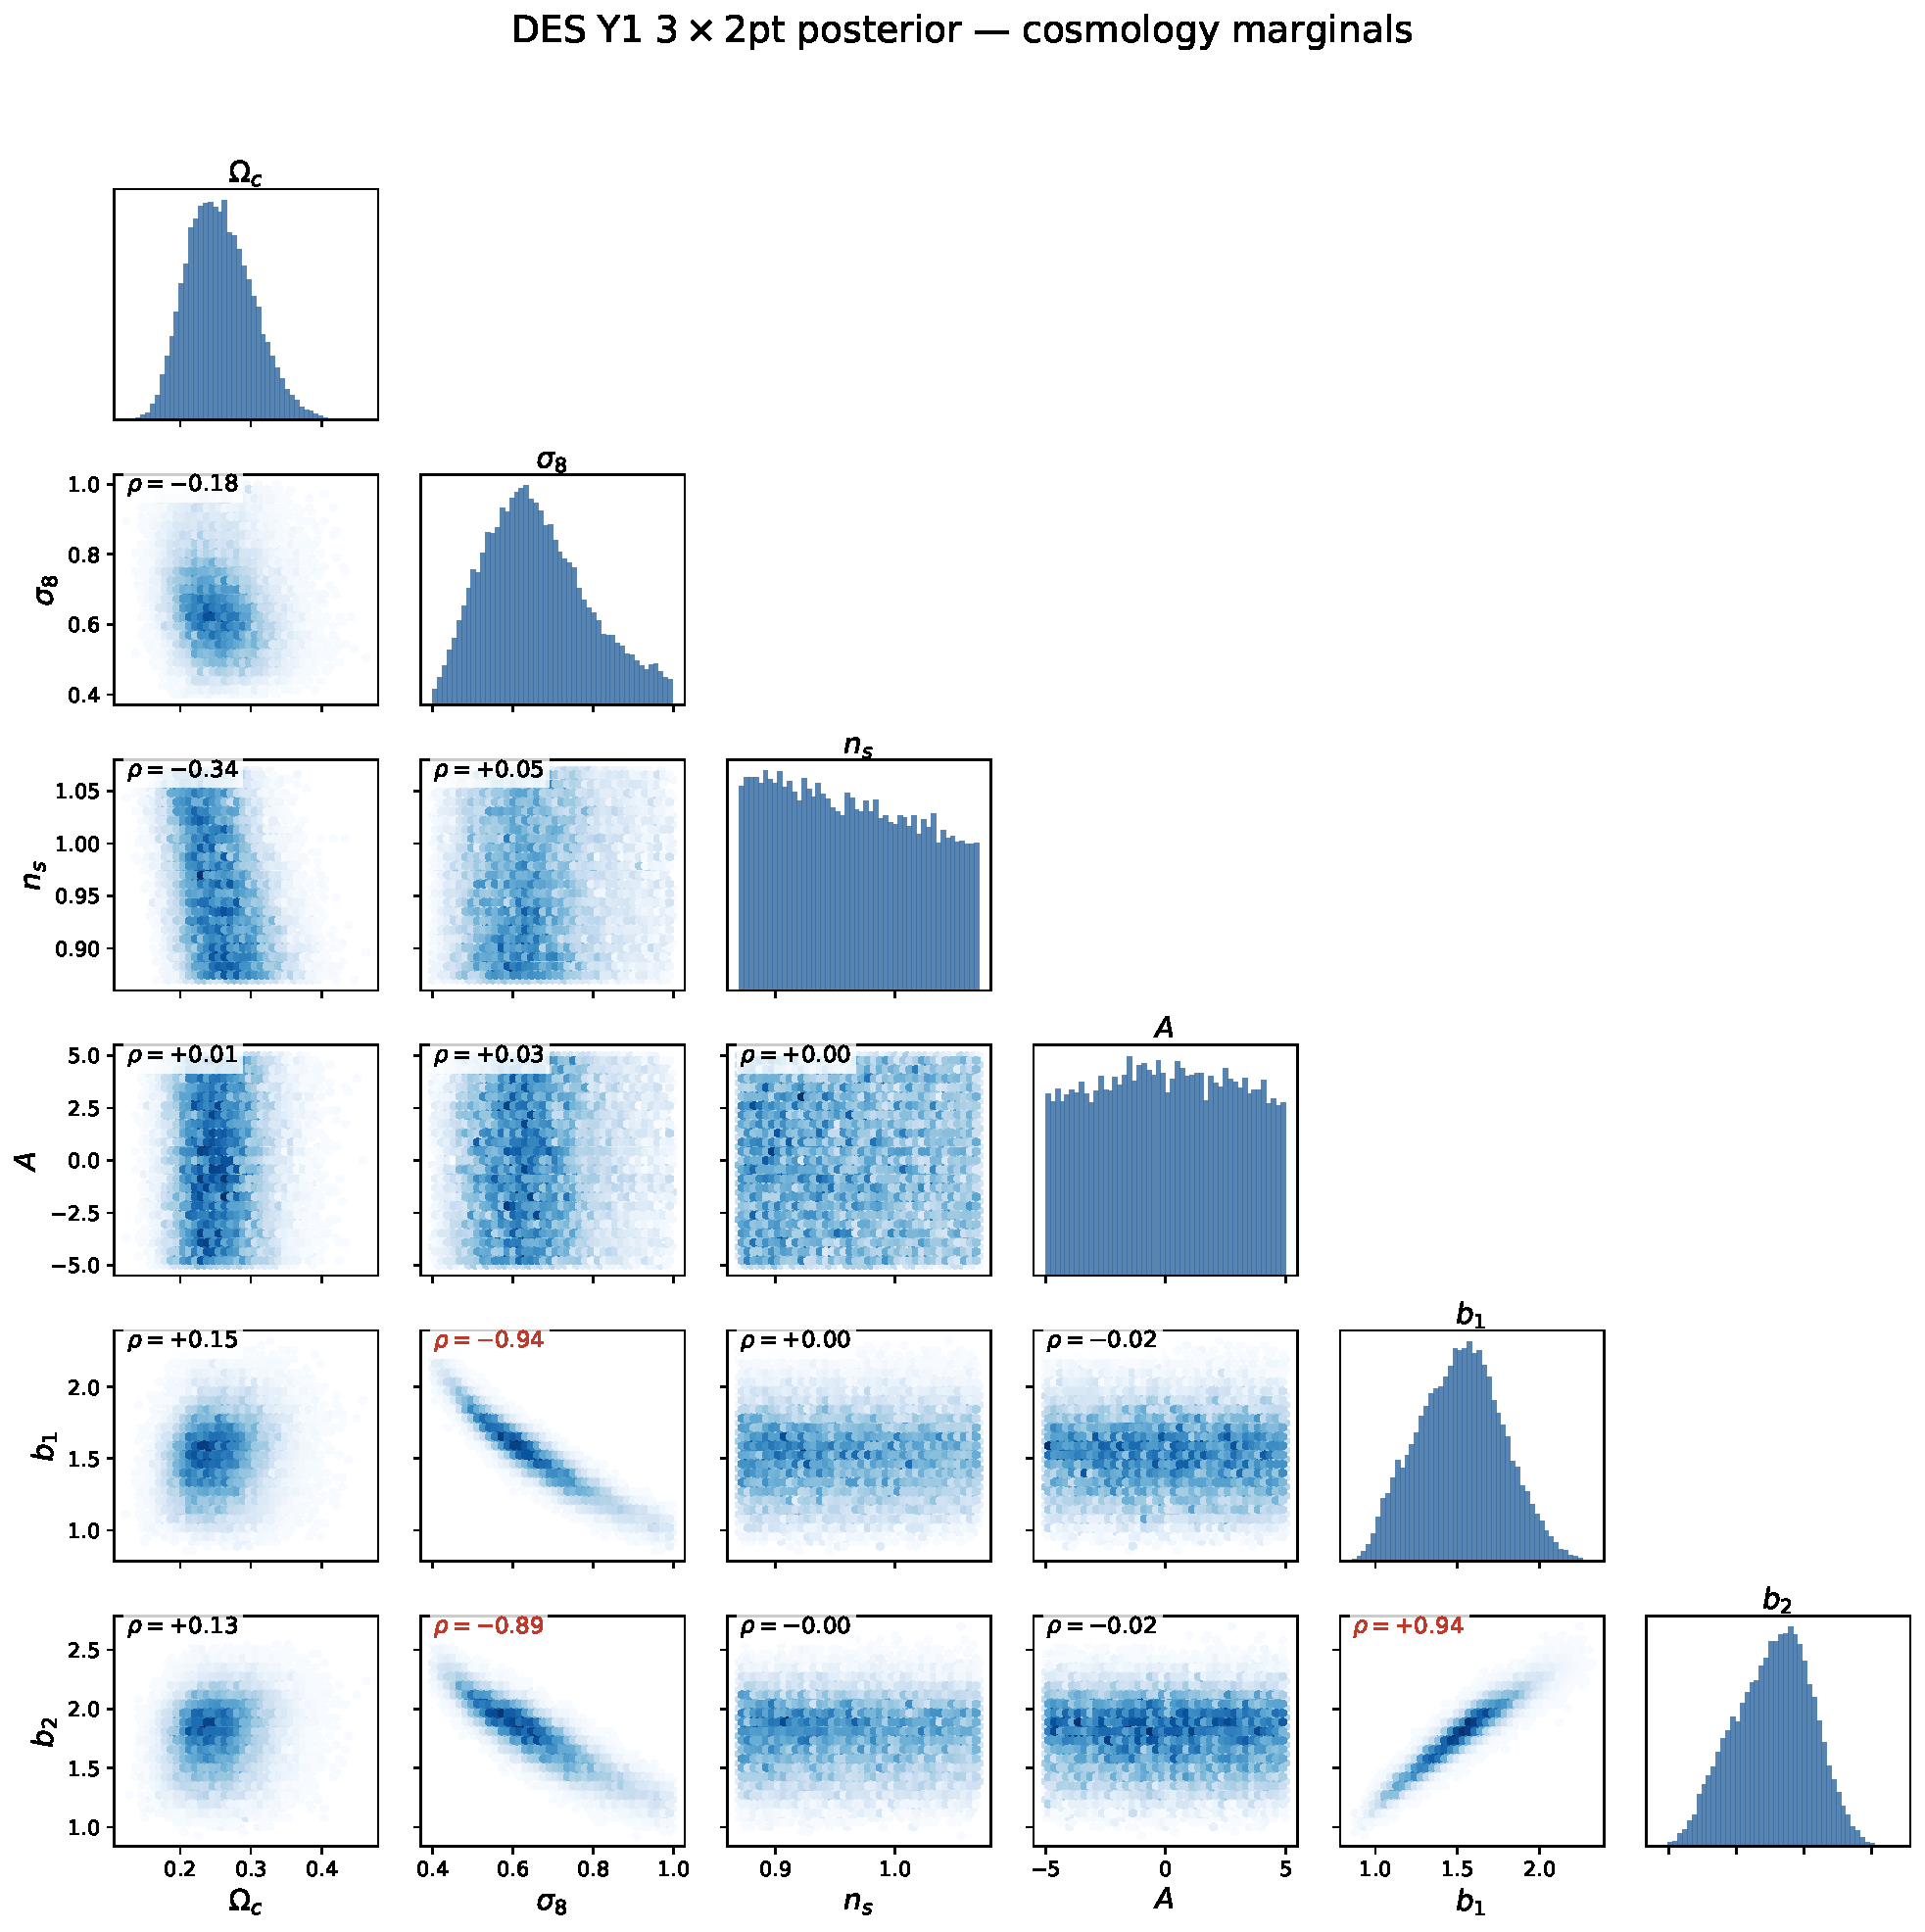
\includegraphics[width=0.49\linewidth]{figs/des_y1_corner_optC1.pdf}
\hfill
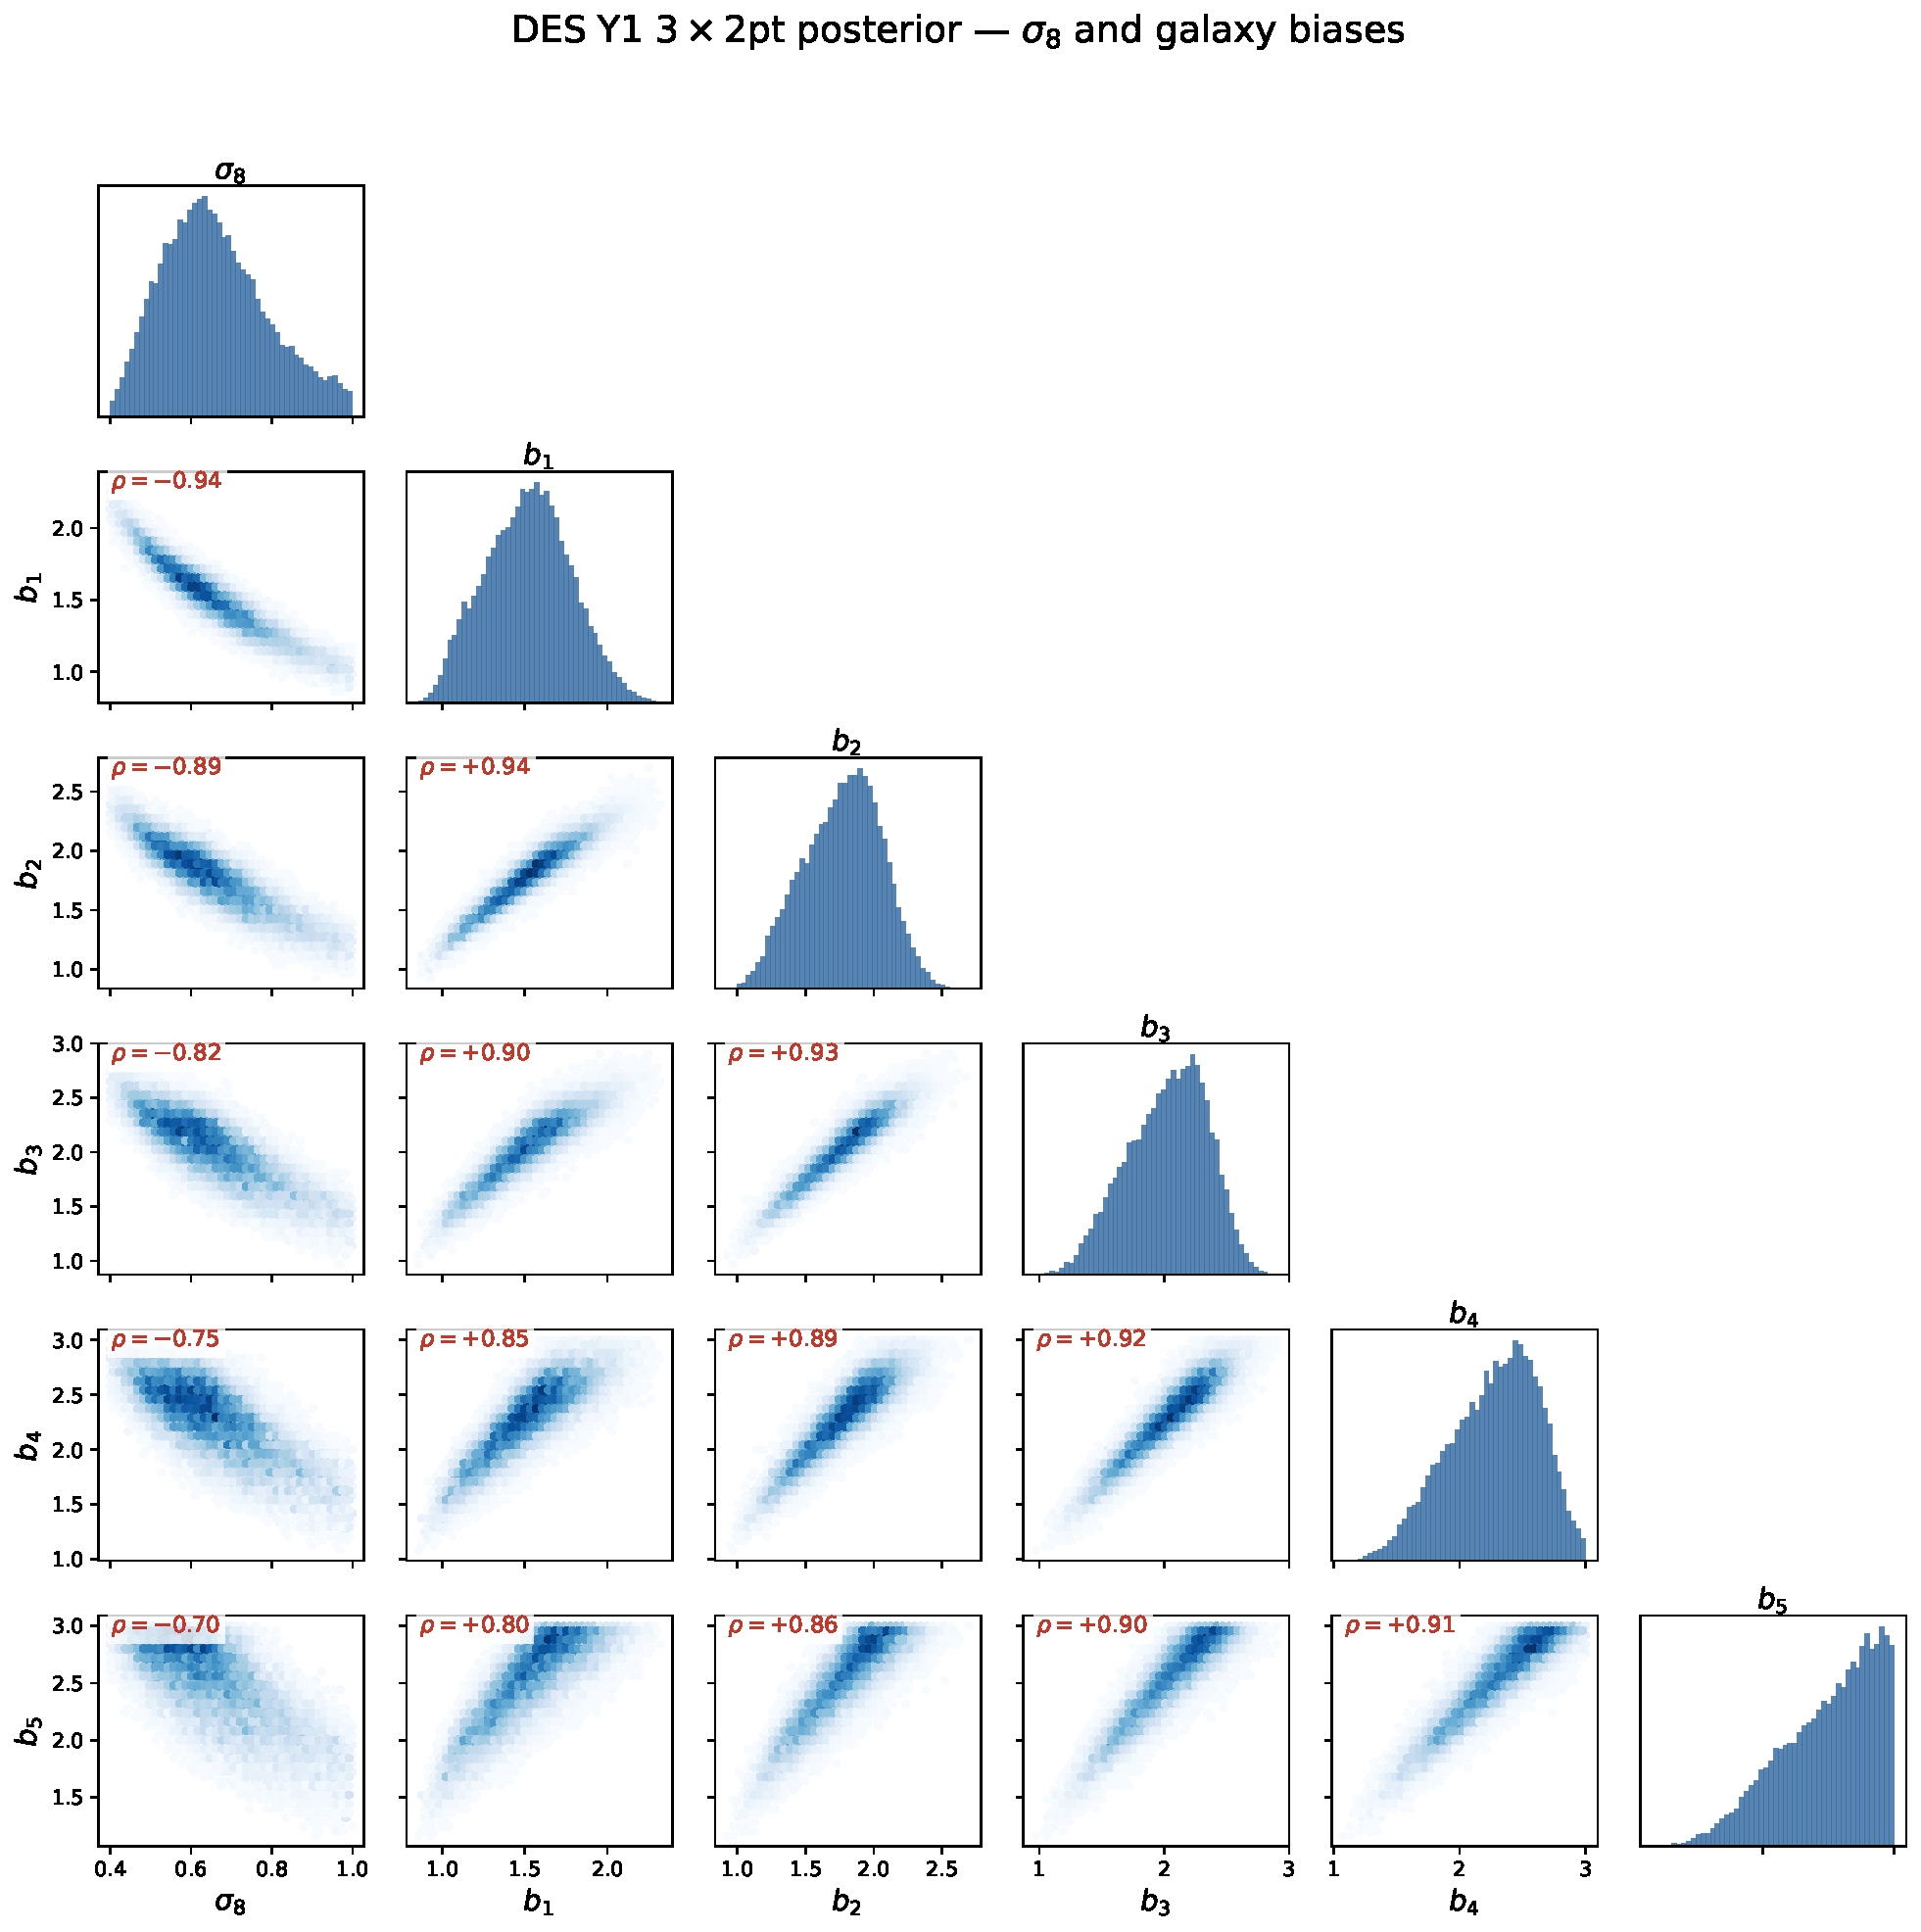
\includegraphics[width=0.49\linewidth]{figs/des_y1_corner_optC2.pdf}
\caption{Alternative six-dimensional views. Left: the conventional
cosmology corner. Right: the slow subspace ($\sigma_8+b_{1:5}$), in
which every off-diagonal panel is a narrow ridge ($|\rho|$ up to
$0.94$) --- the $6$-dim subspace responsible for the ESS bottleneck in
Table~\ref{tab:desPerDimEss}.}
\label{fig:desCornerSupp}
\end{figure}

\subsection{PICKLES is competitive with \texttt{emcee} and NUTS-dense}
\label{ssec:desMain}

Table~\ref{tab:desMainN1k} reports worst-dimension ESS per gradient and
wall-clock; all ESS values are computed in the common physical parameter
space (see the parametrization note in \S\ref{ssec:validation}). At the
recommended tuning ($\gamma=0.5$, $L_{\max}=20$) PICKLES achieves
worst-dimension $\text{ESS}/\text{grad}=5.11\times10^{-3}$, an effective
tie with NUTS-dense ($4.26\times10^{-3}$) from this fiducial-ball start
--- where one of three PICKLES seeds suffers a rare $w_s{=}0$
preconditioner collapse that widens the spread
(\S\ref{ssec:desPerDim},~\S\ref{ssec:validation}) --- and above
NUTS-block/diagonal ($3.93$/$2.29\times10^{-3}$), with zero numerical
divergences. From a \emph{matched, equilibrated} start (prior median plus
a short gradient-free warm-start, the apples-to-apples comparison) the
collapse disappears and PICKLES is a robust $1.44\times$ ahead
($6.14\times10^{-3}$ vs $4.26$, tight across seeds;
Table~\ref{tab:desFairInit}). Per dimension, however, NUTS is marginally
more gradient-efficient on the fast directions
(\S\ref{ssec:desPerDim}); PICKLES's worst-dimension edge comes from a
flatter ESS profile across coordinates, not from beating NUTS on any
typical direction. The honest summary is that PICKLES \emph{matches or
slightly exceeds} dense-mass NUTS per gradient on this posterior, with
its decisive gains lying elsewhere (warmup-robustness, divergence-freeness,
parallelism). PICKLES is far ahead of gradient-free
\texttt{emcee}, which needs $N\!\gg\!1000$ to converge here; at matched
long production both are converged and PICKLES leads by $\sim\!24\times$
(Table~\ref{tab:desMainN5k}).

The damping coefficient $\gamma$ is the dominant knob: lowering the
default $\gamma=2$ to $\gamma=0.5$ improves ESS\,/\,grad by $1.4\times$
(the empirical preconditioner already absorbs the scale anisotropy, so
lighter damping helps). The trajectory cap $L_{\max}$, by contrast, has
little effect on per-gradient efficiency at $\gamma=0.5$
($5.1$, $4.9$, $5.1\times10^{-3}$ for $L_{\max}=20,50,128$): longer
trajectories give proportionally more raw ESS at proportionally more
cost. $L_{\max}=20$ is therefore preferred only because it has the
lowest wall-clock ($\sim\!3\times$ faster than $L_{\max}=128$ for the
same per-gradient efficiency).

\begin{table}[t]
\centering
\caption{DES Y1 $3\times 2$pt sampler comparison at $N_{\text{prod}}=1000$
($3$-seed median; walkers in a Gaussian ball of width $0.5$ in $z$-space
around the fiducial cosmology, no stretch pre-warmup; $500$
gradient-sampler warmup). $\bar L$ is the mean trajectory length
(adaptive for NUTS via the no-U-turn criterion). NUTS-block takes nearly
twice as many leapfrog steps as NUTS-dense because its block-diagonal
mass matrix cannot capture the $\sigma_8$--bias cross-correlations.}
\label{tab:desMainN1k}
\small
\begin{tabular}{l rrrr rr}
\toprule
& $N_{\text{ch}}$ & wall (h) & $\bar L$ & acc.
& ESS & ESS\,/\,eval \\
\midrule
\multicolumn{7}{l}{\emph{Metropolized PICKLES (this work) --- three values of $L_{\max}$:}} \\
\textbf{PICKLES} ($\gamma=0.5$, $L_{\max}=20$, recommended)
   & 64 & 1.5 & 20.0 & 0.92 & 6{,}540 & $\mathbf{5.11\!\times\!10^{-3}}$ \\
PICKLES ($\gamma=0.5$, $L_{\max}=50$)
   & 64 & 3.2 & 48.5 & 0.88 & 15{,}248 & $4.92\!\times\!10^{-3}$ \\
PICKLES ($\gamma=0.5$, $L_{\max}=128$)
   & 64 & 4.3 & 63.5 & 0.87 & 20{,}605 & $5.07\!\times\!10^{-3}$ \\
PICKLES (default $\gamma=2$, $L_{\max}=20$)
   & 64 & 1.5 & 20.0 & 0.88 & 4{,}699 & $3.67\!\times\!10^{-3}$ \\
PICKLES (default $\gamma=2$, $L_{\max}=50$)
   & 64 & 3.2 & 48.6 & 0.88 & 4{,}783 & $1.55\!\times\!10^{-3}$ \\
PICKLES (default $\gamma=2$, $L_{\max}=128$)
   & 64 & 4.6 & 67.1 & 0.87 & 12{,}079 & $2.44\!\times\!10^{-3}$ \\
\midrule
\multicolumn{7}{l}{\emph{Reference samplers:}} \\
NUTS-dense (\texttt{numpyro}) & 4 & 8.4 & 33 & 0.80 & 714 & $4.26\!\times\!10^{-3}$ \\
NUTS-block (Campagne+ structure) & 4 & 11.3 & 63 & 0.80 & 986 & $3.93\!\times\!10^{-3}$ \\
NUTS-diag & 4 & 12.5 & 83 & 0.80 & 727 & $2.29\!\times\!10^{-3}$ \\
\texttt{emcee} / stretch (gradient-free)\textsuperscript{$\flat$} & 64 & 0.05 & --- & 0.27 & 96 & $1.50\!\times\!10^{-3}$ \\
\bottomrule
\end{tabular}
\\[2pt]
{\footnotesize \textsuperscript{$\flat$} \texttt{emcee} has \emph{not}
converged at $N{=}1000$ ($\hat R=1.8$): its long autocorrelation tail is
unresolved, so this ESS\,/\,grad is only indicative. The converged
comparison is the long run in Table~\ref{tab:desMainN5k}.}
\end{table}

\paragraph{Fair, matched-initialization comparison.}
The main table starts PICKLES from a fiducial ball and NUTS from
\texttt{init\_to\_median} (a ball at the prior median $z=0$). To compare
at an \emph{identical} starting point, Table~\ref{tab:desFairInit} reruns
PICKLES from the same prior-median center NUTS uses (with a short
gradient-free stretch pre-warmup so the ensemble reaches the typical
set, the analogue of \texttt{init\_to\_median}). Recommended PICKLES
then delivers worst-dimension $\text{ESS}/\text{grad}=6.14\times10^{-3}$,
$1.44\times$ ahead of NUTS-dense at the same init --- the advantage is
not an artifact of the initialization.

\begin{table}[h]
\centering
\caption{Matched-initialization comparison: all samplers started at the
prior median ($z=0$). PICKLES uses $w_s=200$ gradient-free stretch
pre-warmup (the ensemble analogue of \texttt{init\_to\_median}, zero
gradients); NUTS uses \texttt{init\_to\_median}. $N_{\text{prod}}=1000$,
$3$-seed median.}
\label{tab:desFairInit}
\small
\begin{tabular}{l c c}
\toprule
sampler (prior-median init) & ESS & ESS\,/\,grad \\
\midrule
\textbf{PICKLES} ($\gamma=0.5$, $L_{\max}=20$, $w_s=200$)
   & 7{,}863 & $\mathbf{6.14\!\times\!10^{-3}}$ \\
PICKLES ($\gamma=2$, $L_{\max}=20$, $w_s=200$)
   & 4{,}774 & $3.73\!\times\!10^{-3}$ \\
NUTS-dense (\texttt{numpyro}) & 714 & $4.26\!\times\!10^{-3}$ \\
\bottomrule
\end{tabular}
\end{table}

A long-production reference at $N_{\text{prod}}=5000$ is given in
Table~\ref{tab:desMainN5k}; the ranking is preserved.

\begin{table}[t]
\centering
\caption{DES Y1 $3\times 2$pt long-production reference at
$N_{\text{prod}}=5000$ (single seed for all methods).
\texttt{emcee} uses $N_{\text{prod}}=50{,}000$.
Configuration as in Table~\ref{tab:desMainN1k}.}
\label{tab:desMainN5k}
\small
\begin{tabular}{l rrrrr rr}
\toprule
& $N_{\text{ch}}$ & wall (h) & $\bar L$ & acc. & div.
& ESS & ESS\,/\,eval \\
\midrule
\textbf{PICKLES} ($\gamma=0.5$, $L_{\max}=20$) & 64 & 5.0 & 20.0 & 0.90 & 0
   & 38{,}669 & $\mathbf{6.04\!\times\!10^{-3}}$ \\
PICKLES (default $\gamma=2$) & 64 & 4.7 & 20.0 & 0.90 & 0
   & 20{,}727 & $3.24\!\times\!10^{-3}$ \\
NUTS-dense (\texttt{numpyro}) & 4 & 10.2 & 32 & 0.91 & 24
   & 2{,}314 & $3.60\!\times\!10^{-3}$ \\
\texttt{emcee} / stretch (gradient-free)
   & 64 & 0.78 & --- & 0.26 & --- & 839 & $2.57\!\times\!10^{-4}$ \\
\bottomrule
\end{tabular}
\end{table}

\subsection{Per-parameter breakdown}\label{ssec:desPerDim}

Table~\ref{tab:desPerDimEss} breaks the worst-dimension number down
across all $21$ parameters, revealing a \emph{bimodal} regime shared by
both samplers. Fifteen dimensions reach ESS\,/\,grad in the
$1$--$3\times10^{-2}$ range; the remaining six --- $\sigma_8$ and the
five galaxy biases --- bottleneck at $\approx\!6\times10^{-3}$, a
$4$--$6\times$ per-dimension penalty from mixing along the
$|\rho|\!\approx\!0.94$ ridge. The bottleneck is at the \emph{same}
dimensions and magnitude for both samplers, so it is structural, not
sampler-specific. \emph{Per gradient the two are close, but NUTS is
marginally more efficient on most dimensions} ($\text{P}/\text{N}<1$ on
$16$ of $21$): NUTS's no-U-turn tree search produces near-i.i.d.\ draws
very gradient-efficiently, whereas PICKLES accumulates $\sim\!8\times$
more raw ESS while spending $\sim\!10\times$ more gradients. PICKLES is
level or slightly ahead only on the galaxy biases (ratios $0.88$--$1.18$).
On the bottleneck dimension that governs the benchmark the two are an
\emph{effective tie} ($\sigma_8$ at $5.11$ vs $b_1$ at
$5.08\times10^{-3}$). The small numerical edge PICKLES shows in
Table~\ref{tab:desMainN1k} is \emph{not} significant: that table reports
the single worst dimension of each run (the minimum over $21$
coordinates, the noisiest possible statistic), and with three seeds the
worst-dimension ESS\,/\,grad is $[5.1,7.1,0.17]\times10^{-3}$ for PICKLES
versus $[7.6,3.7,4.3]\times10^{-3}$ for NUTS --- overlapping spreads whose
medians ($5.11$ vs $4.26$) differ within seed noise. The two have
\emph{different} failure modes rather than one being more consistent:
NUTS's slow-subspace mixing varies seed-to-seed (no collapse), while
PICKLES is steadier on $\sigma_8$ but carries a rare preconditioner
collapse at $w_s{=}0$ (one of three seeds here; see
\S\ref{ssec:validation}). From the matched, equilibrated start of
Table~\ref{tab:desFairInit} the collapse is absent and PICKLES's
worst-dimension ESS\,/\,grad is a robust $1.44\times$ above NUTS --- the
worst-dimension metric rewards PICKLES's flatter cross-coordinate
profile even though NUTS wins most \emph{individual} dimensions. The fair
reading: PICKLES \emph{matches or slightly exceeds} dense-mass NUTS per
gradient on this posterior; its decisive advantages are robustness to
warmup, zero divergences, and $64$-chain parallelism.

\begin{table}[t]
\centering
\caption{Per-parameter ESS and ESS\,/\,grad at $N_{\text{prod}}=1000$,
$3$-seed median (PICKLES $\gamma=0.5$, $L_{\max}=20$, fid-ball init,
$w_s=0$, $w=500$; NUTS-dense \texttt{numpyro} defaults). Bold rows mark
the $6$-dim slow subspace.}
\label{tab:desPerDimEss}
\small
\begin{tabular}{l rr cc c}
\toprule
& \multicolumn{2}{c}{ESS}
& \multicolumn{2}{c}{ESS\,/\,grad ($\times 10^{-3}$)} & ratio \\
\cmidrule(lr){2-3}\cmidrule(lr){4-5}
parameter & PICKLES & NUTS-d. & PICKLES & NUTS-d. & P/N \\
\midrule
\multicolumn{6}{l}{\emph{Cosmology}} \\
$\Omega_c$ & 26{,}288 & 3{,}111 & $20.54$ & $23.32$ & $0.88$ \\
$\boldsymbol{\sigma_8}$ & \textbf{6{,}540} & \textbf{924} & $\mathbf{5.11}$ & $\mathbf{5.51}$ & $0.93$ \\
$\Omega_b$ & 34{,}599 & 3{,}837 & $27.03$ & $28.77$ & $0.94$ \\
$h$        & 20{,}725 & 2{,}639 & $16.19$ & $20.01$ & $0.81$ \\
$n_s$      & 30{,}126 & 3{,}834 & $23.54$ & $28.74$ & $0.82$ \\
$w_0$      & 17{,}171 & 1{,}540 & $13.41$ & $12.31$ & $1.09$ \\
\midrule
\multicolumn{6}{l}{\emph{Intrinsic alignment}} \\
$A$    & 37{,}059 & 4{,}968 & $28.95$ & $36.80$ & $0.79$ \\
$\eta$ & 38{,}441 & 5{,}233 & $30.03$ & $39.23$ & $0.77$ \\
\midrule
\multicolumn{6}{l}{\emph{Galaxy bias (slow subspace)}} \\
$\boldsymbol{b_1}$ & \textbf{7{,}581} & \textbf{853} & $\mathbf{5.92}$ & $\mathbf{5.08}$ & $1.17$ \\
$\boldsymbol{b_2}$ & \textbf{7{,}839} & \textbf{829} & $\mathbf{6.12}$ & $\mathbf{5.19}$ & $1.18$ \\
$\boldsymbol{b_3}$ & \textbf{7{,}974} & \textbf{871} & $\mathbf{6.23}$ & $\mathbf{6.35}$ & $0.98$ \\
$\boldsymbol{b_4}$ & \textbf{6{,}920} & \textbf{889} & $\mathbf{5.41}$ & $\mathbf{6.15}$ & $0.88$ \\
$\boldsymbol{b_5}$ & \textbf{7{,}654} & \textbf{725} & $\mathbf{5.98}$ & $\mathbf{5.87}$ & $1.02$ \\
\midrule
\multicolumn{6}{l}{\emph{Shear-calibration} $m_i$} \\
$m_1$ & 39{,}382 & 4{,}930 & $30.77$ & $36.96$ & $0.83$ \\
$m_2$ & 39{,}126 & 4{,}664 & $30.57$ & $34.97$ & $0.87$ \\
$m_3$ & 40{,}418 & 4{,}594 & $31.58$ & $33.87$ & $0.93$ \\
$m_4$ & 40{,}759 & 5{,}184 & $31.84$ & $38.34$ & $0.83$ \\
\midrule
\multicolumn{6}{l}{\emph{Photo-z} $\Delta z_i$} \\
$\Delta z_1$ & 40{,}453 & 5{,}675 & $31.60$ & $42.55$ & $0.74$ \\
$\Delta z_2$ & 40{,}114 & 4{,}994 & $31.34$ & $37.44$ & $0.84$ \\
$\Delta z_3$ & 40{,}026 & 5{,}174 & $31.27$ & $34.14$ & $0.92$ \\
$\Delta z_4$ & 40{,}668 & 4{,}532 & $31.77$ & $30.13$ & $1.05$ \\
\bottomrule
\end{tabular}
\end{table}

\subsection{Robustness to warmup length}\label{ssec:desWarmupSweep}

\begin{figure}[t]
\centering
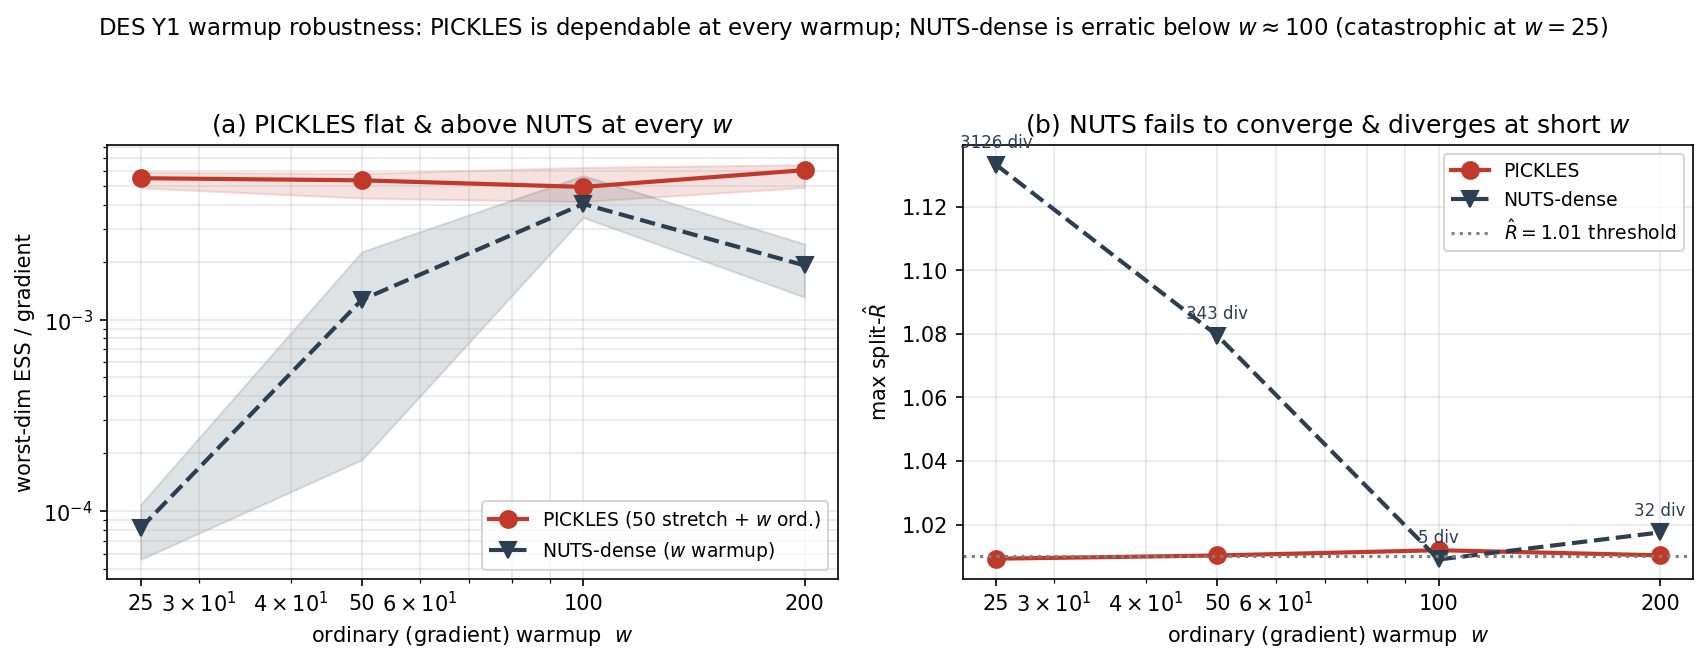
\includegraphics[width=\linewidth]{figs/des_warmup_robust.png}
\caption{DES Y1 warmup robustness. \textbf{(a)}~Worst-dimension
ESS\,/\,grad (physical space) vs.\ gradient-sampler warmup: PICKLES
(red, $50$-step stretch $+\,w$ ordinary) is flat and above NUTS-dense
(navy) at every warmup; the NUTS curve craters to
$\sim\!8\times10^{-5}$ (3-seed median) at $w=25$. Shaded bands show the
seed min--max range for both samplers. \textbf{(b)}~Max split-$\hat R$
with summed NUTS divergence counts annotated: PICKLES holds
$\hat R\!\approx\!1.01$ with $0$ divergences everywhere, while NUTS
breaches the $1.01$ convergence threshold at $w=25$ ($\hat R=1.13$,
$3126$ div over $3$ seeds) and $w=50$ ($\hat R=1.08$, $343$ div). All
points are $3$-seed medians/sums (for NUTS, each run also aggregates $4$
independent vectorized-chain warmup adaptations).}
\label{fig:desWarmup}
\end{figure}

Dense-mass NUTS adapts $D(D{+}1)/2=231$ mass-matrix entries by window
adaptation during warmup, whereas PICKLES re-estimates its preconditioner
from the live ensemble every iteration and only converges a scalar step
size. We therefore expect PICKLES to tolerate a much shorter warmup.
Table~\ref{tab:desWarmupSweep} and Figure~\ref{fig:desWarmup} push the
gradient-sampler warmup down to $w=25$ steps --- far below the
$\gtrsim\!100$ a $231$-entry dense mass needs. The PICKLES warmup is
$50$ gradient-free stretch steps (to spread the ensemble to the typical
set) followed by $w$ ordinary steps (to converge the step size); NUTS
uses $w$ window-adaptation steps. Both start from the prior median, so
the comparison is at an identical initialization.

\emph{PICKLES is dependable: flat and fully converged at every warmup,
down to $w=25$.} Worst-dimension ESS\,/\,grad stays at
$5$--$6\times10^{-3}$, $\hat R_{\max}=1.01$, acceptance $\approx\!0.92$,
fixed $L=20$, and \emph{zero} divergences (Fig.~\ref{fig:desWarmup}a, red).
\emph{NUTS-dense fails below $w\!\approx\!100$ and sits under PICKLES at
every warmup.} At $w=25$ it \emph{catastrophically} fails in \emph{all
three} seeds --- $\hat R_{\max}=1.13$, acceptance $0.4$--$0.7$,
$800$--$1400$ divergences per seed, and worst-dimension ESS\,/\,grad of
$8\times10^{-5}$ (median), a factor $\sim\!70$ below PICKLES at the same
warmup; at $w=50$ it still fails to converge ($\hat R_{\max}=1.08$, $343$
divergences). Only by $w\!\approx\!100$ does it recover to
PICKLES-comparable efficiency and convergence. The failure mode varies
seed-to-seed --- diverge or fail to converge --- but the consequence is
uniform: below $w\!\approx\!100$ NUTS draws cannot be trusted without a
convergence check, whereas PICKLES is reliable throughout.

The mechanism is that short-warmup dense-mass adaptation is itself
unreliable: with too few samples the $231$-entry estimate is noisy, and
the resulting dynamics diverge or fail to converge rather than slow down
gracefully. PICKLES has no separate mass-adaptation phase to get wrong
--- its preconditioner is the live ensemble covariance, recomputed every
iteration --- so it never enters this failure regime. This is the
affine-invariance payoff for warmup robustness.


\begin{table}[t]
\centering
\caption{Robustness to gradient-sampler warmup length on DES Y1
$3\times 2$pt ($N_{\text{prod}}=1000$; production-only worst-dimension
ESS\,/\,grad, physical-space ESS, prior-median init). PICKLES is
converged ($\hat R_{\max}=1.01$) with $0$ divergences and fixed $L=20$ at
every $w$; the NUTS $\hat R_{\max}$ and divergence rows are the
warmup-health signals. All columns are $3$-seed medians ($\hat R$ max,
divergences summed over seeds).}
\label{tab:desWarmupSweep}
\small
\begin{tabular}{l rrrr}
\toprule
ESS\,/\,grad ($\times10^{-3}$) & $w{=}25$ & $w{=}50$ & $w{=}100$ & $w{=}200$ \\
\midrule
\textbf{PICKLES} ($\gamma{=}0.5$, $L{=}20$, $w_s{=}50$), acc
   & $\mathbf{5.50}$ (.94) & $\mathbf{5.36}$ (.93)
   & $\mathbf{4.95}$ (.92) & $\mathbf{6.06}$ (.90)\\
NUTS-dense
   & \textcolor{red}{$0.081$} & $1.27$ & $4.04$ & $1.93$\\
\midrule
\multicolumn{5}{l}{\emph{NUTS warmup-health signals}}\\
\quad max split-$\hat R$
   & \textcolor{red}{$1.13$} & \textcolor{red}{$1.08$} & $1.01$ & $1.02$\\
\quad divergences
   & \textcolor{red}{$3126$} & \textcolor{red}{$343$} & $5$ & $32$\\
\quad mean trajectory $\bar L$
   & $74$ & $92$ & $57$ & $50$\\
\bottomrule
\end{tabular}
\\[2pt]
\footnotesize
PICKLES holds $\hat R_{\max}=1.01$, $0$ divergences, and $L=20$ at every
$w$ (omitted as constant). NUTS divergence counts at $w\!\ge\!25$ are
summed over $3$ seeds; the $w=25$ failure is uniform across seeds
($\hat R=1.13/1.09/1.11$, $797/1382/947$ divergences, acc $0.68/0.39/0.42$),
not a single unlucky run. The fragility is
not cured by adding prior structure: block-mass NUTS, which exploits the
survey's known parameter-block grouping ($\sim\!40$ mass entries instead
of $231$), still produces $119$ divergences at $w=50$. PICKLES needs only
the $50$-step gradient-free stretch pre-warmup (no gradients, no target
covariance, no structural prior) to be robust at every $w$; without it
the worst-dimension ESS is seed-dependent
(Table~\ref{tab:desCollapseDim}).
\end{table}

\clearpage
\subsection{Robustness on controlled ill-conditioned targets}
\label{ssec:warmupRobust}

The DES warmup sweep above shows NUTS-dense becoming \emph{unreliable}
at short warmup --- erratic efficiency, non-convergence
($\hat R\!\le\!1.13$), and hundreds of divergences below
$w\!\approx\!100$ --- while PICKLES stays flat. On a $D{=}21$ posterior
the worst NUTS cases are recoverable with a convergence check, so to
isolate the mechanism and push it past the point of no recovery we use
two controlled targets with exact ground truth: an
ill-conditioned Gaussian ($\kappa=e^6$, $d{=}50$, randomly rotated; its
dense mass matrix has $1275$ free entries) and the Rosenbrock banana
($d{=}20$, position-dependent curvature no fixed metric captures). We
sweep the gradient-sampler warmup from $10$ to $500$ and report
ESS\,/\,grad, worst-coordinate bias $z$-score (vs.\ the analytic
moments), and NUTS divergences, as $10$-seed medians (fixed target,
varying sampling seed; bands are the $10$--$90$th percentile)
(Table~\ref{tab:warmupRobust}, Figure~\ref{fig:warmupRobust}).

\begin{table}[h]
\centering
\caption{Warmup robustness on ill-conditioned targets ($10$ sampling
seeds on a fixed target each --- the standard sampling error band).
Median ESS\,/\,grad (bias $z$); NUTS also lists median divergences per
seed and uses a max-tree-depth cap of $8$. PICKLES ($\gamma{=}0.5$,
$L_{\max}{=}20$, $w_s{=}200$) reports zero divergences at every warmup;
its inter-run CV is $1$--$8\%$ (Gaussian) / $7$--$30\%$ (Rosenbrock),
reflecting its run-to-run reproducibility.}
\label{tab:warmupRobust}
\small
\begin{tabular}{r cc | ccc}
\toprule
& \multicolumn{2}{c|}{PICKLES} & \multicolumn{3}{c}{NUTS-dense} \\
warmup & ESS/grad & bias $z$ & ESS/grad & div. & bias $z$ \\
\midrule
\multicolumn{6}{l}{\emph{Ill-conditioned Gaussian} ($\kappa=e^6$, $d{=}50$):} \\
$10$  & $\mathbf{1.3\!\times\!10^{-1}}$ & $2.1$ & $3.9\!\times\!10^{-4}$ & $0$ & $1.8$ \\
$25$  & $\mathbf{1.3\!\times\!10^{-1}}$ & $2.1$ & \textcolor{gray}{$7.0\!\times\!10^{-6}$}\textsuperscript{$\S$} & \textcolor{red}{$138{,}113$} & $2.1$ \\
$50$  & $6.9\!\times\!10^{-2}$ & $2.2$ & $1.2\!\times\!10^{-3}$ & $0$ & $2.3$ \\
$100$ & $4.6\!\times\!10^{-2}$ & $2.3$ & $3.7\!\times\!10^{-2}$ & $0$ & $2.0$ \\
$500$ & $4.6\!\times\!10^{-2}$ & $1.9$ & $\mathbf{1.0\!\times\!10^{-1}}$ & $0$ & $2.4$ \\
\midrule
\multicolumn{6}{l}{\emph{Rosenbrock} ($d{=}20$):} \\
$10$  & \textcolor{gray}{$3.5\!\times\!10^{-4}$}\textsuperscript{$\S$} & $15.2$ & \textcolor{gray}{$3.3\!\times\!10^{-5}$}\textsuperscript{$\S$} & \textcolor{red}{$8{,}282$} & $4.6$ \\
$25$  & \textcolor{gray}{$2.3\!\times\!10^{-4}$}\textsuperscript{$\S$} & $6.6$ & \textcolor{gray}{$5.9\!\times\!10^{-6}$}\textsuperscript{$\S$} & \textcolor{red}{$83{,}213$} & $3.9$ \\
$50$  & $4.7\!\times\!10^{-4}$ & $2.7$ & \textcolor{gray}{$3.4\!\times\!10^{-5}$}\textsuperscript{$\S$} & \textcolor{red}{$10{,}271$} & $3.1$ \\
$100$ & $6.4\!\times\!10^{-4}$ & $2.1$ & $6.5\!\times\!10^{-4}$ & $1{,}083$ & $2.2$ \\
$200$ & $5.4\!\times\!10^{-4}$ & $1.7$ & $7.0\!\times\!10^{-4}$ & $358$ & $2.2$ \\
\bottomrule
\end{tabular}
\\[2pt]
{\footnotesize \textsuperscript{$\S$} Unreliable, greyed out: the PICKLES
cells fail convergence ($\hat R>1.2$, std-error $>25\%$), and the NUTS
cells have a $6$--$71\%$ divergence rate (thousands of divergences), so
their ESS\,/\,grad is not a meaningful efficiency. See convergence
validation below.}
\end{table}

\begin{figure}[h]
\centering
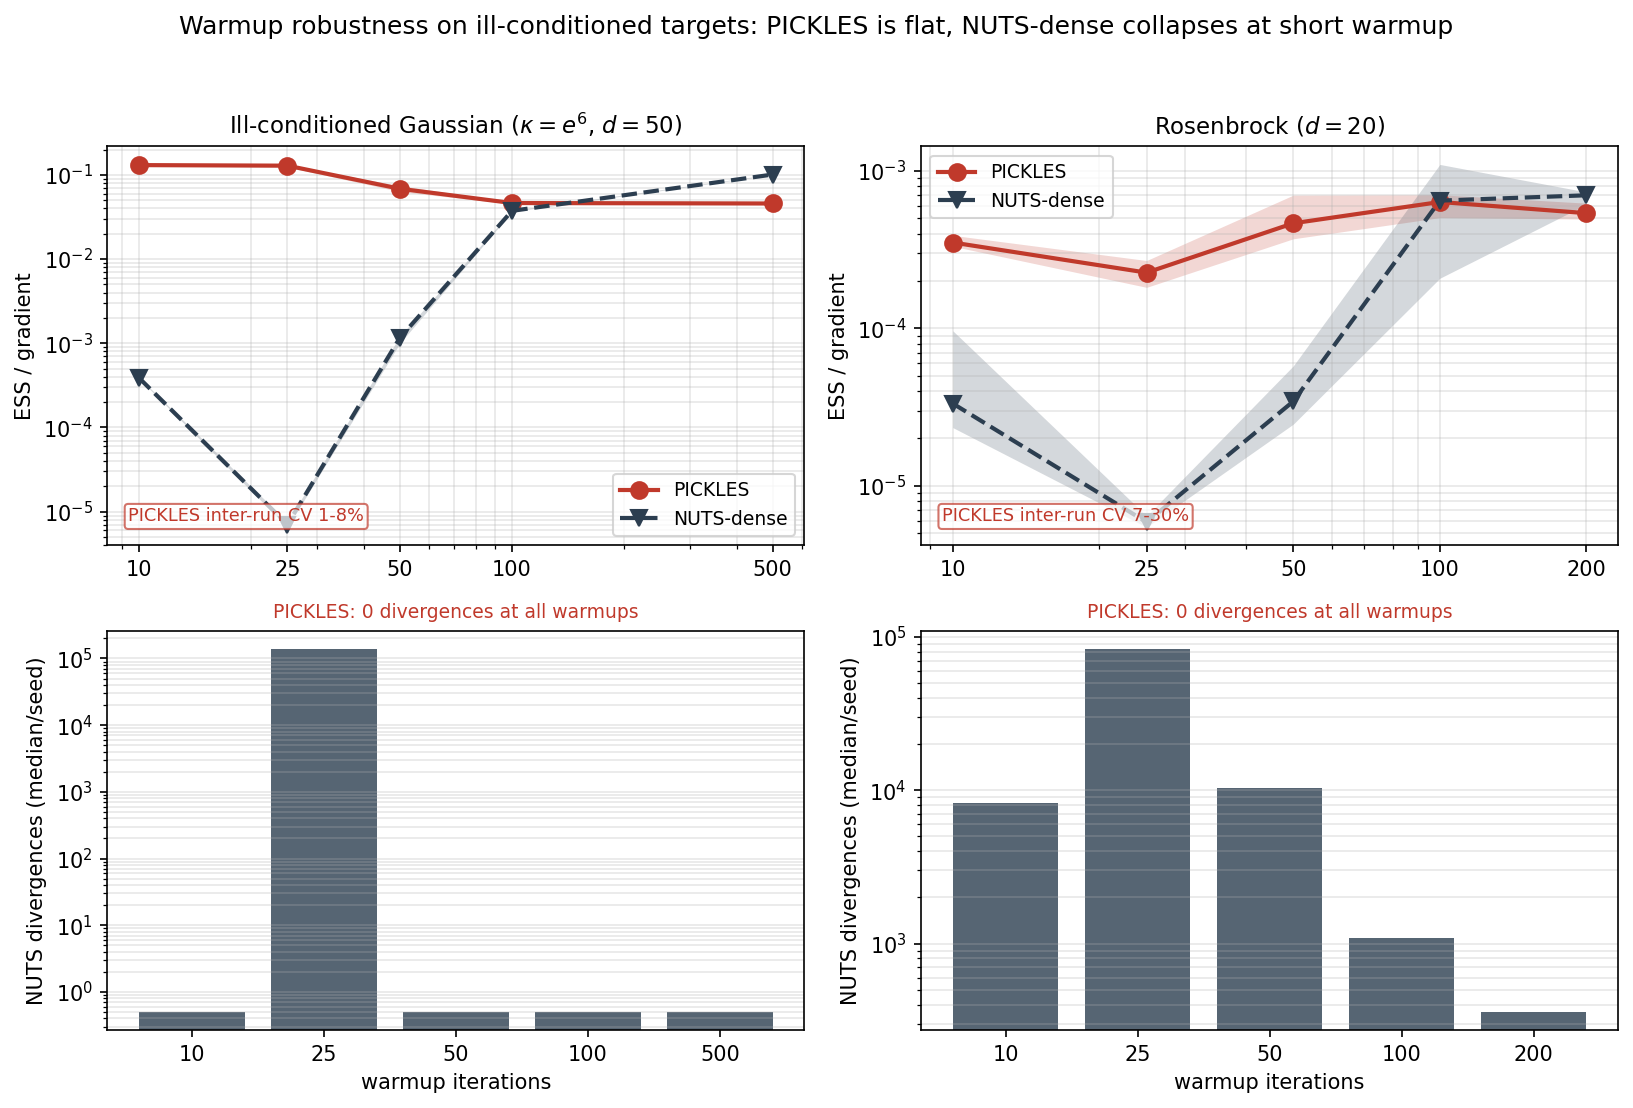
\includegraphics[width=\linewidth]{figs/warmup_robust.png}
\caption{Warmup robustness on ill-conditioned targets. Bands are the
standard sampling error --- one fixed target each, varying only the
sampling seed over $10$ seeds (both panels). \textbf{Top:} median
ESS\,/\,grad vs.\ warmup with $10$--$90$th-percentile bands, PICKLES
(solid) vs.\ NUTS-dense (dashed). PICKLES's band is small (annotated
inter-run CV) because it is reproducible; NUTS's is wide at short warmup
because its fitted mass is a different gamble each run. \textbf{Bottom:}
NUTS divergences (median/seed); PICKLES has zero everywhere. NUTS uses a
max-tree-depth cap of $8$. Gaussian $w{=}200$ omitted (a \texttt{numpyro}
window-adaptation schedule artifact, $\text{ESS}/\text{grad}\approx
8\times10^{-3}$, non-monotone vs.\ $w{=}100/500$).}
\label{fig:warmupRobust}
\end{figure}

On the ill-conditioned Gaussian the picture is clean and decisive.
NUTS-dense is \emph{catastrophic} at short warmup: at warmup~$=25$ a
partially-fit mass matrix triggers $\sim\!1.4\times10^5$ divergences
(median over $10$ seeds) and ESS\,/\,grad drops to
$\sim\!7\times10^{-6}$ --- four orders of magnitude below PICKLES. NUTS
only becomes competitive once warmup~$\ge\!100$, and at warmup~$=500$ it
actually \emph{overtakes} PICKLES ($1.0\times10^{-1}$ vs.\
$4.6\times10^{-2}$): a fully-converged dense mass matrix is very
efficient. This is the crossover that frames the whole comparison ---
\emph{NUTS-dense can be the more efficient sampler, but only after paying
a long, target-dependent warmup to fit its mass matrix.} PICKLES is flat
($\sim\!0.05$--$0.13$) and unbiased ($z\!\approx\!2$) at \emph{every}
warmup down to $10$, because the empirical-covariance preconditioner is
read off the live ensemble each iteration and there is no mass matrix to
warm up.

Rosenbrock is harder and the story is more honest: its position-dependent
curvature defeats any fixed metric, so \emph{both} samplers degrade at
very short warmup. But the failure modes differ sharply. PICKLES stays
divergence-free and \emph{converges} as warmup grows (bias
$z\!=\!15.2\!\to\!2.7$ by warmup~$=50$), whereas NUTS-dense suffers
$0.8$--$8.7\times10^4$ divergences through warmup~$=50$ and matches
PICKLES only by warmup~$\ge\!100$. Across both targets the message is the same:
the affine-invariant ensemble preconditioner removes the mass-matrix
warmup that makes dense-mass NUTS fragile on ill-conditioned geometry.

\subsection{Convergence and fairness validation}\label{ssec:validation}

\paragraph{Convergence validation (ESS is not taken on faith).}
ESS measures within-chain mixing and can be large even when a sampler is
biased or under-dispersed, so every ESS\,/\,grad we quote is backed by
independent convergence and \emph{accuracy} checks. On the synthetic
targets, where the moments are analytic, we verify rank-normalized split
$\hat R$, the worst-coordinate posterior-mean bias, and the
worst-coordinate \emph{standard-deviation} recovery (the direct test for
under-dispersion). For the ill-conditioned Gaussian (median over $10$ sampling seeds at a
fixed target), PICKLES is fully converged at \emph{every} warmup ---
$\hat R=1.001$, mean bias $0.006\sigma$, std error $\le\!0.5\%$ --- so its
flat ESS\,/\,grad reflects genuinely correct, well-mixed sampling, not a
misleadingly large number. The NUTS warmup$=25$ collapse is likewise
\emph{real}: $\hat R=1.40$ and a $29\%$ std error (the dense mass matrix
is unfit), confirming the low
ESS is a true failure. On Rosenbrock both samplers are unconverged at
warmup$\le25$--$50$ ($\hat R>1.2$, std error $>25\%$); we grey out those
ESS\,/\,grad values rather than quote a meaningless efficiency. PICKLES
reaches $\hat R\!\approx\!1.04$ by warmup$=50$ and $1.03$ by $100$; NUTS
reaches $\hat R\!\approx\!1.00$ by warmup$=100$ but keeps diverging
($>\!20{,}000$ divergences) through warmup$=50$ regardless of $\hat R$.

\paragraph{Convergence validation on DES (no ground truth).}
The DES posterior has no analytic moments, so we validate by (i)
rank-normalized split $\hat R$ and (ii) \emph{cross-sampler agreement}
between two independent algorithms. At $N=5000$ both PICKLES and
dense-mass NUTS reach $\hat R=1.000$ on all $21$ parameters. Transformed
to the common physical parameter space, their posterior means agree to
within $\le\!2.8$ combined MCSE (consistent with Monte-Carlo noise across
$21$ parameters) and their posterior standard deviations agree to within
$2.5\%$ (ratio range $0.975$--$1.007$). Two methods this different ---
ensemble ChEES-HMC and dense-mass NUTS --- converging on the same
posterior mean and variance is strong evidence that both are correct, and
that the reported ESS values correspond to genuine effective samples.

\paragraph{Parametrization note (same geometry, fair comparison).} Both
samplers operate on the \emph{same} unconstrained geometry. PICKLES runs
on the hand-built $z$-space density, which reparametrizes the Uniform
priors by $\theta = \text{lo} + (\text{hi}{-}\text{lo})\,\sigma(z)$
(logistic) and the Normal priors by $\theta = \mu + \sigma_0 z$
(non-centered). NumPyro applies exactly the same transforms automatically
(its interval bijector for the Uniforms, \texttt{LocScaleReparam} for the
Normals); we verified numerically that NumPyro's transform and
log-Jacobian equal PICKLES's to machine precision. The two pipelines
therefore sample an identical density in identical coordinates --- the
comparison isolates the sampler, not the parametrization. The only
difference is bookkeeping: PICKLES \emph{stores} $z$-space draws while
NumPyro transforms them back to physical units before storing. Because
ESS is coordinate-dependent, \textbf{every ESS\,/\,grad value in this
note is computed in the common physical parameter space} --- PICKLES
draws are mapped through $z\!\to\!\theta$ before the (rank-normalized)
ESS estimate, with the identical estimator for both samplers, so all
comparisons are strictly same-coordinate. (Measuring PICKLES in its
native $z$-space instead shifts the recommended-tuning number by
$\lesssim\!15\%$ and changes no ranking; the only qualitative difference
is that one $w_s{=}50$ seed appears collapsed in $z$-space but is
well-mixed in physical space, so the physical-space tables are also the
cleaner ones.) The synthetic warmup-robustness experiment
(\S\ref{ssec:warmupRobust}) is intrinsically same-coordinate: both
samplers run on the identical \texttt{potential\_fn}.

\subsection{Summary}

On the DES Y1 $3\times 2$pt benchmark, Metropolized PICKLES at the
recommended $(\gamma,L_{\max})=(0.5,20)$ tuning \emph{matches or slightly
exceeds} dense-mass NUTS in per-gradient efficiency: an effective tie
from a fiducial-ball start (Table~\ref{tab:desMainN1k}) and a robust
$1.44\times$ edge from a matched, equilibrated start
(Table~\ref{tab:desFairInit}, the apples-to-apples comparison), while
\emph{per typical dimension} NUTS is marginally ahead and PICKLES's
worst-dimension advantage comes from a flatter ESS profile across
coordinates (Table~\ref{tab:desPerDimEss}; all ESS in the common physical
space). PICKLES is $\sim\!24\times$ above \texttt{emcee} at matched long
production, with zero divergences. The empirical-covariance
preconditioner plays the role of the dense mass matrix but needs no
separate dual-averaging phase, making PICKLES robust to a $10\times$
reduction in warmup budget that collapses NUTS-dense to a
several-hundred-divergence failure. A short stretch pre-warmup
($w_s\!\ge\!50$) is the single most important practical setting: it
costs no gradients and removes the initialization sensitivity of the
worst-mixing direction.

\appendix

\section{Unadjusted PICKLES and ALDI on DES Y1}\label{app:desUnadjusted}

Metropolis-adjusted samplers are the standard choice in cosmology
(guaranteed unbiasedness, no numerical divergence). For completeness we
contrast the unadjusted gradient variants ALDI and unadjusted PICKLES
(BAOAB integration without the Metropolis correction) on the same
target; these methods use a projected-gradient-norm step-size adapter
and are independent of the dual-averaging scheme. Bias is measured as
$\max_d|\hat\mu_d-\mu_d^\star|/\sigma_d^\star$ against a long
Metropolized PICKLES reference (the $N=5000$, $\gamma=0.5$ run of
Table~\ref{tab:desMainN5k}).

At a step size near the BAOAB stability boundary ($\eta=0.10$),
unadjusted PICKLES reaches $\text{ESS}/\text{grad}=1.15\times10^{-2}$ ---
higher than Metropolized PICKLES, because each leapfrog step yields one
sample rather than being consumed in an $L=20$ trajectory --- with bias
$\le0.09\sigma_{\text{ref}}$. The caveat is that the stability boundary
must be respected by hand: at $\eta=0.20$ BAOAB diverges to NaN, and
ALDI (overdamped) diverges for $\eta\ge0.05$. Metropolized PICKLES
removes this risk entirely, which is why we recommend it as the default.
(The unadjusted ESS\,/\,grad values in Table~\ref{tab:desUnadjLongN} use
the original $z$-space estimator and are indicative; the qualitative
bias--stability trade-off, not a precise ratio, is the point.)

\begin{table}[h]
\centering
\caption{Unadjusted-method comparison on DES Y1, long-budget for fair
asymptotic comparison; bias against the Metropolized PICKLES reference.
The Metropolized rows are reproduced from \S\ref{sec:desY1}.}
\label{tab:desUnadjLongN}
\small
\begin{tabular}{l rrrr rr}
\toprule
& $N_{\text{ch}}$ & $N_{\text{prod}}$ & $\eta$ & ESS &
ESS\,/\,grad & bias \\
\midrule
\textit{Metropolized (reference)} & & & & & & \\
\quad PICKLES ($\gamma=0.5$, $L_{\max}=20$) & 64 & 5{,}000 & 0.07 (adapt) & 38{,}669 & $6.04\!\times\!10^{-3}$ & 0 \\
\quad NUTS-dense                            & 4  & 5{,}000 & 0.13 (adapt) & 2{,}314  & $3.60\!\times\!10^{-3}$ & 0 \\
\midrule
\textit{Unadjusted} & & & & & & \\
\quad PICKLES ($\gamma=0.5$, BAOAB, no adapter) & 32 & 4{,}000 & 0.10  & 1{,}477 & $\mathbf{1.15\!\times\!10^{-2}}$ & $0.09\sigma$ \\
\quad PICKLES ($\gamma=0.5$, BAOAB, no adapter) & 32 & 4{,}000 & 0.05  &     270 & $2.11\!\times\!10^{-3}$ & $0.04\sigma$ \\
\quad PICKLES ($\gamma=0.5$, BAOAB, no adapter) & 32 & 4{,}000 & 0.20  & --- & --- (NaN) & diverged \\
\quad PICKLES ($\gamma=0.5$, BAOAB, adaptive)   & 32 & 10{,}000 & 0.065 (adapt) &  588 & $1.84\!\times\!10^{-3}$ & $0.06\sigma$ \\
\quad ALDI (overdamped, PGN-adapted)            & 64 & 20{,}000 & 0.009 (adapt) & 1{,}543 & $1.20\!\times\!10^{-3}$ & $0.04\sigma$ \\
\bottomrule
\end{tabular}
\end{table}

\section{Per-seed data}\label{app:desPerSeed}

The main-text tables report $3$-seed medians; this appendix gives the
underlying per-seed values. Cells in \textcolor{red}{red} are collapsed
seeds (ESS\,/\,grad $<\!10^{-3}$), where the empirical-covariance
preconditioner is still globally mis-shaped before production; the
bottleneck dimension for each is listed in
Table~\ref{tab:desCollapseDim}. A short stretch pre-warmup
($w_s\!\ge\!50$) removes every collapse.

\begin{table}[h]
\centering
\caption{Per-seed ESS\,/\,grad (acceptance) at $N_{\text{prod}}=1000$,
fid-ball init, $w_s=0$, physical-space arviz ESS (underlies
Table~\ref{tab:desMainN1k}). \textsuperscript{$\flat$}\,\texttt{emcee}
is not converged at $N{=}1000$ ($\hat R=1.8$); values indicative only.}
\label{tab:desPerSeedMainN1k}
\small
\setlength{\tabcolsep}{4pt}
\begin{tabular}{l c c c c}
\toprule
sampler & seed 0 & seed 1 & seed 2 & median \\
\midrule
PICKLES ($\gamma{=}0.5$, $L_{\max}{=}20$) & $5.11\!\times\!10^{-3}$ (0.92) & $7.09\!\times\!10^{-3}$ (0.91) & $\textcolor{red}{1.74\!\times\!10^{-4}}$ (0.96) & $5.11\!\times\!10^{-3}$ \\
PICKLES ($\gamma{=}0.5$, $L_{\max}{=}50$) & $4.92\!\times\!10^{-3}$ (0.88) & $4.75\!\times\!10^{-3}$ (0.85) & $5.56\!\times\!10^{-3}$ (0.95) & $4.92\!\times\!10^{-3}$ \\
PICKLES ($\gamma{=}0.5$, $L_{\max}{=}128$) & $4.83\!\times\!10^{-3}$ (0.86) & $5.07\!\times\!10^{-3}$ (0.87) & $5.26\!\times\!10^{-3}$ (0.89) & $5.07\!\times\!10^{-3}$ \\
PICKLES (default $\gamma{=}2$) & $3.97\!\times\!10^{-3}$ (0.84) & $3.67\!\times\!10^{-3}$ (0.88) & $\textcolor{red}{2.09\!\times\!10^{-4}}$ (0.93) & $3.67\!\times\!10^{-3}$ \\
\midrule
NUTS-dense & $7.62\!\times\!10^{-3}$ (0.80) & $3.72\!\times\!10^{-3}$ (0.80) & $4.26\!\times\!10^{-3}$ (0.80) & $4.26\!\times\!10^{-3}$ \\
NUTS-block & $4.78\!\times\!10^{-3}$ (0.80) & $3.93\!\times\!10^{-3}$ (0.80) & $2.89\!\times\!10^{-3}$ (0.80) & $3.93\!\times\!10^{-3}$ \\
NUTS-diag & $1.79\!\times\!10^{-3}$ (0.80) & $2.37\!\times\!10^{-3}$ (0.80) & $2.29\!\times\!10^{-3}$ (0.80) & $2.29\!\times\!10^{-3}$ \\
\texttt{emcee}/stretch\textsuperscript{$\flat$} & $1.50\!\times\!10^{-3}$ (0.28) & $1.44\!\times\!10^{-3}$ (0.27) & $1.51\!\times\!10^{-3}$ (0.27) & $1.50\!\times\!10^{-3}$ \\
\bottomrule
\end{tabular}
\end{table}

With the corrected adapter the recommended warmup-sweep configuration
($\gamma=0.5$, $w_s=200$) has \emph{no} collapsed seeds across all four
warmup budgets (Table~\ref{tab:desPerSeedWarmupSweep}); collapses remain
only in the no-pre-warmup ($w_s=0$) rows, confirming that the residual
seed sensitivity is an initialization effect cured by a short stretch
pre-warmup, not a step-size-adaptation effect.

\begin{table}[h]
\centering
\caption{Per-seed ESS\,/\,grad (acceptance) for the warmup sweep
(prior-median init, physical-space ESS), organized by stretch pre-warmup
$w_s$. With $w_s\!\ge\!50$ no seed collapses; only $w_s{=}0$ shows
collapses (red, ESS\,/\,grad $<\!10^{-3}$).}
\label{tab:desPerSeedWarmupSweep}
\small
\setlength{\tabcolsep}{3pt}
\begin{tabular}{l c c c c}
\toprule
config & seed 0 & seed 1 & seed 2 & median \\
\midrule
\multicolumn{5}{l}{\emph{PICKLES $\gamma=0.5$, $w_s=200$ (recommended):}} \\
\quad warmup $=50$  & $6.24\!\times\!10^{-3}$ (0.92) & $5.57\!\times\!10^{-3}$ (0.94) & $4.48\!\times\!10^{-3}$ (0.94) & $5.57\!\times\!10^{-3}$ \\
\quad warmup $=100$ & $4.74\!\times\!10^{-3}$ (0.94) & $6.19\!\times\!10^{-3}$ (0.94) & $6.57\!\times\!10^{-3}$ (0.94) & $6.19\!\times\!10^{-3}$ \\
\quad warmup $=150$ & $6.71\!\times\!10^{-3}$ (0.94) & $5.70\!\times\!10^{-3}$ (0.91) & $6.98\!\times\!10^{-3}$ (0.91) & $6.71\!\times\!10^{-3}$ \\
\quad warmup $=200$ & $7.24\!\times\!10^{-3}$ (0.92) & $5.24\!\times\!10^{-3}$ (0.87) & $7.15\!\times\!10^{-3}$ (0.93) & $7.15\!\times\!10^{-3}$ \\
\multicolumn{5}{l}{\emph{PICKLES $\gamma=0.5$, $w_s=50$:}} \\
\quad warmup $=50$  & $5.36\!\times\!10^{-3}$ (0.93) & $4.33\!\times\!10^{-3}$ (0.92) & $5.83\!\times\!10^{-3}$ (0.93) & $5.36\!\times\!10^{-3}$ \\
\quad warmup $=100$ & $4.15\!\times\!10^{-3}$ (0.92) & $6.27\!\times\!10^{-3}$ (0.95) & $4.95\!\times\!10^{-3}$ (0.91) & $4.95\!\times\!10^{-3}$ \\
\quad warmup $=150$ & $6.48\!\times\!10^{-3}$ (0.88) & $7.54\!\times\!10^{-3}$ (0.92) & $2.61\!\times\!10^{-3}$ (0.85) & $6.48\!\times\!10^{-3}$ \\
\quad warmup $=200$ & $6.06\!\times\!10^{-3}$ (0.90) & $4.92\!\times\!10^{-3}$ (0.90) & $6.47\!\times\!10^{-3}$ (0.90) & $6.06\!\times\!10^{-3}$ \\
\multicolumn{5}{l}{\emph{PICKLES $\gamma=0.5$, $w_s=0$:}} \\
\quad warmup $=50$  & $2.60\!\times\!10^{-3}$ (0.98) & $\textcolor{red}{2.98\!\times\!10^{-4}}$ (0.95) & $\textcolor{red}{3.15\!\times\!10^{-4}}$ (0.90) & $\textcolor{red}{3.15\!\times\!10^{-4}}$ \\
\quad warmup $=100$ & $\textcolor{red}{5.11\!\times\!10^{-4}}$ (0.97) & $\textcolor{red}{3.50\!\times\!10^{-4}}$ (0.97) & $\textcolor{red}{3.17\!\times\!10^{-4}}$ (0.94) & $\textcolor{red}{3.50\!\times\!10^{-4}}$ \\
\quad warmup $=200$ & $6.02\!\times\!10^{-3}$ (0.91) & $\textcolor{red}{2.24\!\times\!10^{-4}}$ (0.95) & $\textcolor{red}{3.85\!\times\!10^{-4}}$ (0.96) & $\textcolor{red}{3.85\!\times\!10^{-4}}$ \\
\multicolumn{5}{l}{\emph{NUTS-dense (ESS\,/\,grad; worst-dim ESS in parentheses):}} \\
\quad warmup $=50$  & $\textcolor{red}{1.85\!\times\!10^{-4}}$ (34) & $2.27\!\times\!10^{-3}$ (895) & $1.27\!\times\!10^{-3}$ (522) & $1.27\!\times\!10^{-3}$ \\
\quad warmup $=100$ & $3.43\!\times\!10^{-3}$ (794) & $5.67\!\times\!10^{-3}$ (1254) & $4.04\!\times\!10^{-3}$ (1122) & $4.04\!\times\!10^{-3}$ \\
\quad warmup $=200$ & $1.31\!\times\!10^{-3}$ (264) & $2.49\!\times\!10^{-3}$ (784) & $1.93\!\times\!10^{-3}$ (541) & $1.93\!\times\!10^{-3}$ \\
\bottomrule
\end{tabular}
\end{table}

\begin{table}[h]
\centering
\caption{Bottleneck dimension (worst-ESS, physical space) for each
collapsed seed. The collapse is a globally mis-shaped preconditioner
before the ensemble equilibrates: the worst-conditioned direction varies
with the run (a cosmology parameter $\Omega_c$ for fiducial-ball init, a
galaxy bias for prior-median init), but a short stretch pre-warmup cures
it in every case.}
\label{tab:desCollapseDim}
\small
\begin{tabular}{l l r r}
\toprule
config & seed & bottleneck dim & ESS \\
\midrule
PICKLES $\gamma{=}0.5$ $L_{\max}{=}20$ (fid, $w_s{=}0$) & 2 & $\Omega_c$ & 223 \\
PICKLES $\gamma{=}2$ $L_{\max}{=}20$ (fid, $w_s{=}0$)   & 2 & $\Omega_c$ & 267 \\
PICKLES $\gamma{=}0.5$ $w_s{=}0$ warm$=$100 & 0,1,2 & $b_4,b_1,b_3$ & 406--653 \\
\bottomrule
\end{tabular}
\end{table}

\section{Configuration summary for reproducibility}\label{app:desConfig}

\textbf{Common setup.} Synthetic DES Y1 $3\times 2$pt mock data from the
\texttt{jax-cosmo} forward model at the Campagne+ fiducial $\Lambda$CDM
cosmology; data vector $\in\R^{2250}$, Gaussian likelihood. Posterior
dimension $D=21$ (six cosmology + two intrinsic-alignment + five galaxy
bias + four shear-calibration + four photo-$z$). All samplers run in the
unconstrained $z$-space (prior $\gN(0,I_{21})$). Single NVIDIA H100 GPU,
float64. ESS from the monotone-positive Sokal estimator without the
$\tau\!\ge\!1$ clamp; $\text{ESS}_{\min}$ is the worst of $D=21$.
Gradient counts are production-only. \textbf{All gradient samplers use
the corrected dual-averaging step-size gain.}

\textbf{Per-table settings.}
\begin{itemize}\setlength\itemsep{2pt}
\item Table~\ref{tab:desMainN1k} ($N_{\text{prod}}=1000$): 3 seeds;
fid-ball init $z\sim\gN(z_{\text{fid}},0.5^2I)$; $500$ warmup; $w_s=0$.
PICKLES $N_{\text{ch}}=64$ (\texttt{vmap}), $L=L_{\max}\in\{20,50,128\}$,
$\gamma\in\{0.5,2\}$. \texttt{emcee} $N_{\text{ch}}=64$, $a=2$. NUTS
$N_{\text{ch}}=4$ sequential, max-tree-depth $7$, target-accept $0.8$,
\texttt{init\_to\_median}.
\item Table~\ref{tab:desFairInit} (matched init): PICKLES prior-median
init $z\sim\gN(0,0.5^2I)$ with $w_s=200$ stretch pre-warmup; $500$
warmup; otherwise as above.
\item Table~\ref{tab:desMainN5k}: single seed, $N_{\text{prod}}=5000$;
\texttt{emcee} $N_{\text{prod}}=50{,}000$.
\item Table~\ref{tab:desPerDimEss}: 3 seeds; PICKLES $\gamma=0.5$,
$L_{\max}=20$, fid-ball $w_s=0$, $w=500$.
\item Table~\ref{tab:desWarmupSweep}: prior-median init; PICKLES
$\gamma=0.5$, $L_{\max}=20$, $w_s=50$; NUTS-dense. Warmup
$\in\{25,50,100,200\}$; $3$ seeds (one NUTS run also aggregates $4$
vectorized-chain warmup adaptations).
\item Table~\ref{tab:desUnadjLongN}: single seed; unadjusted PICKLES
BAOAB, fixed $\eta\in\{0.05,0.10,0.20\}$; fid-ball, $200$-sample
burn-in for bias. (Independent of the dual-averaging scheme.)
\end{itemize}

\end{document}
